\begin{frame}[fragile]{Деревья термов}
\begin{definition}[]
\emph{Деревья (термов с метапеременными)} -- это деревья (или даже DAGи), где 
\begin{enumerate}
\item в узлах находятся $n$-местные "функциональные символы"
\item у узлов $n$ поддеревьев
\item в листьях могут стоять \emph{метапеременные}
\end{enumerate}
\end{definition}
\vspace{1em}

\begin{center}
\begin{tikzpicture}[->,thick,scale=0.5, every node/.style={scale=0.5}
  , grow via three points={
      one child at (0,-2) and 
      two children at (.8,-2) and (-0.8,-2) 
  }]
     \tikzstyle{tnode}=[circle, inner sep=1.5mm]
     \tikzstyle{var}=[ circle, inner sep=1.5mm,draw]
     \def\rstep{5cm}
     \huge
         
    \begin{scope}[xshift= \rstep]
      \node[tnode] {f}
          child {node[tnode] {g} 
            child {node[var] {x} }
            child {node[tnode] {a} }
          }
          child[missing] {} 
          child {node[tnode] {g} 
            child {node[var] {x} }
            child {node[tnode] {a} }
          };
%        child[missing] {} ;
      \end{scope}
      
    \begin{scope}[xshift=15cm]
      \node[tnode] {f}
          child {node[tnode] (gggg) {g} 
            child[missing] {node[var] {x} }
            child {node[tnode]  {a} }
          }
          child[missing] {}
          child {node[tnode]  {g} 
            child {node[var]  (xxxx) {x} }
            child {node[tnode] {a} }
          };

      \draw [->,thick](gggg.south)
              to [out=-90,in=90] (2,-5)
              to [out=-90,in=0] (1,-6) 
              to [out=180,in=-45]  (xxxx.south); 
      \end{scope}
      
      \begin{scope}[xshift=23cm]
        \node[tnode] (ffff) {f}
            child {node[tnode] (gggg) {g} 
              child {node[var] {x} }
              child {node[tnode] {a} }
            };

        \draw [->,thick](ffff)
                to [out=0,in=90] (1,-1)
                to [out=-90,in=45]  (gggg.east); 
        \end{scope}
 \end{tikzpicture}
\end{center}
\end{frame}

\begin{frame}[fragile]{Подстановка}
\begin{definition}
Подстановка -- это отображение имён метапеременных в деревья
\end{definition}

\begin{definition}[Применение подстановки $\sigma$ к дереву]
Замена в дереве всех переменных $v\in Dom(\sigma)$  на $\sigma(v)$
\end{definition}

\begin{minipage}[b]{0.2\linewidth}
\begin{center}
\begin{tikzpicture}[->,thick,scale=0.5, every node/.style={scale=0.5}
  , grow via three points={
      one child at (0,-2) and 
      two children at (.8,-2) and (-0.8,-2) 
  }]
     \tikzstyle{tnode}=[circle, inner sep=1.5mm]
     \tikzstyle{var}=[ circle, inner sep=1.5mm,draw]
     \def\rstep{5cm}
     \huge
         
    \begin{scope}[xshift= \rstep]
      \node[tnode] {f}
          child {node[tnode] {g} 
            child {node[tnode] {a} }
            child {node[var] {x} }
          }
          child[missing] {}
          child {node[var] {y}
          };
      \end{scope}
\end{tikzpicture}
Исходное дерево
\end{center}

\end{minipage}
\hspace{1cm}
\begin{minipage}[b]{0.35\linewidth}
  \begin{equation*}
    \sigma(v) =
    \begin{cases}
      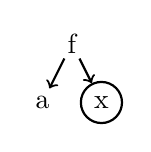
\begin{tikzpicture}[->,thick,scale=0.5, every node/.style={scale=1}]
          \tikzstyle{tnode}=[circle, inner sep=.5mm]
          \tikzstyle{var}=[ circle, inner sep=1mm,draw]
          \node[tnode] {f}
                    child {node[tnode] {a} }
                    child {node[var] {x} 
                    };
      \end{tikzpicture}, & \text{if}\ v=y \\%[5pt]
            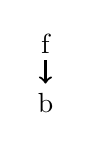
\begin{tikzpicture}[->,thick,scale=0.5, every node/.style={scale=1}]
                \tikzstyle{tnode}=[circle, inner sep=.5mm]
                \tikzstyle{var}=[ circle, inner sep=1mm,draw]
                \node[tnode] {f}
                            child {node[tnode] {b} }
                          ;
            \end{tikzpicture}, & \text{if}\ v= z
    \end{cases}
  \end{equation*}
  Подстановка c $Dom(\sigma) = \{y, z\}$
\end{minipage}
\hspace{.5cm}
\begin{minipage}[b]{0.3\linewidth}
\begin{center}
\begin{tikzpicture}[->,thick,scale=0.5, every node/.style={scale=0.5}
  , grow via three points={
      one child at (0,-2) and 
      two children at (.8,-2) and (-0.8,-2) 
  }]
     \tikzstyle{tnode}=[circle, inner sep=1.5mm]
     \tikzstyle{var}=[ circle, inner sep=1.5mm,draw]
     \def\rstep{5cm}
     \huge
         
    \begin{scope}[xshift= \rstep]
      \node[tnode] {f}
          child {node[tnode] {g} 
            child {node[tnode] {a} }
            child {node[var] {x} }
          }
          child[missing] {}
          child {node[tnode] {f}
                  child {node[var] {x} }
                  child {node[tnode] {a} }
          };
      \end{scope}
\end{tikzpicture}

Дерево после подстановки
\end{center}
\end{minipage}
\end{frame}

\begin{frame}
\begin{definition}[Более общая подстановка]
Подстановка $\sigma_0$ более общая, чем $\sigma$, если последнюю можно получить из первой путём специализации(сужения) более общей $\sigma_0$ на некоторых входах
\end{definition}
\vspace{1em}

Примеры:
\begin{itemize}
\item Подстановка $\{x\mapsto y, y\mapsto z\}$ более общая чем $\{x\mapsto 1, y\mapsto 1\}$, т.к. её можно сузить с помощью $z\mapsto 1$
%\item Подстановка $\{x\mapsto y, z\mapsto 1\}$ более общая чем $\{x\mapsto y, y\mapsto 1\}$, т.к. её можно сузить с помощью $y\mapsto 1$
\item Подстановки $\{y\mapsto 1\}$ и $\{z\mapsto y\}$ не являются более общими друг к другу
\end{itemize}
\end{frame}


\begin{frame}
\begin{definition}[Задача (синтаксической) унификации]
Даны два дерева с метапеременными. Необходимо подобрать наиболее общую подстановку-унификатор (\emph{most general unifier}, mgu) так, чтобы после её применения два дерева стали одинаковыми. Или же сказать, что mgu не существует.
\end{definition}
\end{frame}


\begin{frame}{Алгоритм синтаксической унификации}
\vspace{1em}
\textbf{Вход}: два дерева и стартовая подстановка $\sigma$.\\
\textbf{Выход}: подстановка-унификатор или её отсутствие.\\

Во время алгоритма синхронно обходим два дерева
\begin{itemize}
\item Унифицируем (мета)переменную $x\in Dom(\sigma)$, тогда надо вместо $x$ унифицировать $\sigma(x) \equiv \text{walk}(\sigma, x)$
\item Унифицируем (мета)переменную $x$ и дерево $\mathcal{V}$, но $\text{check}(\sigma,x,\mathcal{V})\equiv \text{false}$, т.е. не можем расширить подстановку  --- унификация не возможна
\item Если можем расширить подстановку, то выдаем ответ: $ \text{extend}(\sigma,x,\mathcal{V})$
\item Два разных функциональных символа -- унификация не возможна 
\item Иначе (два одинаковых функц. символа с одинаковой арностью $n$) мы попарно унифицируем аргументы, "протягивая" текущую подстановку через $n$ рекурсивных вызовов
\end{itemize}

\end{frame}


\begin{frame}[fragile]{Упражнение 1}
Задача: можно ли передать значения типа \mlinline{'a list -> ('a -> 'b) -> 'b } туда, где ожидается значение типа \mlinline{'c list -> ('c -> 'd list) -> 'd list}?
\vspace{1em}

\begin{minipage}{0.45\linewidth}
\begin{tikzpicture}[->,thick,scale=0.5, every node/.style={scale=0.5}
  , grow via three points={
      one child at (0,-2) and 
      two children at (.8,-2) and (-0.8,-2) 
  }]
     \tikzstyle{tnode}=[rectangle, inner sep=1.5mm]
     \tikzstyle{var}=[ circle, inner sep=1.5mm,draw]
     \def\rstep{5cm}
     \huge
         
    \begin{scope}[xshift= \rstep]
      \node[tnode] {\mlinline{->}}
          child {node[tnode] {\mlinline{->}} 
            child { node [tnode] {\mlinline{->}}
                        %child{ node [tnode] {\mlinline{list}} 
                        child { node[var] {\mlinline{'b}} }
                        child[missing] {}
                        %}
                       }
            child[missing] {}
            child { node [tnode] {\mlinline{->}}
                    child { node[var] {\mlinline{'b}} }
                    child { node[var] {\mlinline{'a}} }
                   }
          }
          child[missing] {}
            child{ node [tnode] {\mlinline{list}} 
              child[missing] {}
               child { node[var] {\mlinline{'a}} }
            };
      \end{scope}
\end{tikzpicture}
\end{minipage}\hspace{1cm}
\begin{minipage}{0.45\linewidth}
\begin{tikzpicture}[->,thick,scale=0.5, every node/.style={scale=0.5}
  , grow via three points={
      one child at (0,-2) and 
      two children at (.8,-2) and (-0.8,-2) 
  }]
     \tikzstyle{tnode}=[rectangle, inner sep=1.5mm]
     \tikzstyle{var}=[ circle, inner sep=1.5mm,draw]
     \def\rstep{5cm}
     \huge
         
    \begin{scope}[xshift= \rstep]
      \node[tnode] {\mlinline{->}}
          child {node[tnode] {\mlinline{->}} 
            child { node [tnode] {\mlinline{->}}
                        child{ node [tnode] {\mlinline{list}} 
                          child { node[var] {\mlinline{'d}} }
                        }
                       }
            child[missing] {}
            child { node [tnode] {\mlinline{->}}
                    child{ node [tnode] {\mlinline{list}} 
                      child { node[var] {\mlinline{'d}} }
                    }
                    child { node[var] {\mlinline{'c}} }
                   }
          }
          child[missing] {}
            child{ node [tnode] {\mlinline{list}} 
              child[missing] {}
               child { node[var] {\mlinline{'c}} }
            };
      \end{scope}
\end{tikzpicture}
\end{minipage}
\end{frame}


\begin{frame}[fragile]{Упражнение 2}
Проунифицировать $f(\alpha,\beta)$ и $f(l(\beta), n)$, где $\alpha,\beta$ -- метапеременные.
\vspace{1em}

\begin{minipage}{0.45\linewidth}
  \begin{center}
  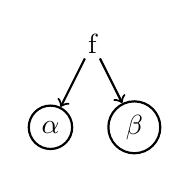
\begin{tikzpicture}[->,thick,scale=.71, every node/.style={scale=1}]
      \tikzstyle{tnode}=[circle, inner sep=.5mm]
      \tikzstyle{var}=[ circle, inner sep=1mm,draw]
      \node[tnode] {f}
                child {node[var] {$\alpha$} }
                child {node[var] {$\beta$} 
                };
  \end{tikzpicture}
  \end{center}
\end{minipage}\hspace{1cm}
\begin{minipage}{0.45\linewidth}
  \begin{center}
  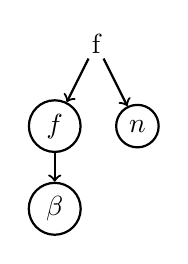
\begin{tikzpicture}[->,thick,scale=.7, every node/.style={scale=1}]
  \tikzstyle{tnode}=[circle, inner sep=.5mm]
  \tikzstyle{var}=[ circle, inner sep=1mm,draw]
  \node[tnode] {f}
      child {
        node[var] {$f$}
        child {node[var] {$\beta$} }
      }
      child {node[var] {$n$} 
      };
  \end{tikzpicture}
  \end{center}
\end{minipage}
\vspace{1em}\pause

На выходе можно полученную подстановку записывать двумя способами:\\

\begin{minipage}[t]{0.45\linewidth}
\begin{center}
"Треугольная"
\begin{align*}
  \alpha &\mapsto f(\beta)\\
  \beta &\mapsto n
\end{align*} 
\end{center}
\end{minipage}\hspace{1cm}
\begin{minipage}[t]{0.45\linewidth}
\begin{center}
"Идемпотентная"
\begin{align*}
  \alpha &\mapsto f(n)\\
  \beta &\mapsto n
\end{align*} 
\end{center}
\end{minipage}
\end{frame}


\begin{frame}{Треугольная и идемпотентная подстановки}
\begin{center}
\begin{tabular}{ |>{\centering\arraybackslash}p{5cm}|>{\centering\arraybackslash}p{3cm}|>{\centering\arraybackslash}p{5cm}| } 
 \hline
 Треугольная & Название & Идемпотентная \\ \hline
 {$ \begin{aligned}
   \alpha &\mapsto f(\beta)\\
   \beta &\mapsto n
 \end{aligned}$}  & Пример & {$\begin{aligned}
   \alpha &\mapsto f(n)\\
   \beta &\mapsto n
 \end{aligned}  $} \\  \hline
 
 Зависит от значений других ключей & Значение $\sigma(x)$ & $\sigma(x)$ -- окончательный образ $x$ \\ \hline
  экспоненциальная* & Сложность операции \mlinline{walk} & константная*\\  \hline
  константная* & Сложность операции \mlinline{extend} & экспоненциальная*\\  \hline
\end{tabular}
\end{center}
\end{frame}

\begin{frame}[fragile]{Упражнение\uncover<3->{. Occurs check}}

Проунифицируйте  $f(x, y)$ и $y$.\pause

\begin{center}
Будет ошибка или
\begin{tikzpicture}[->,thick,scale=0.5, every node/.style={scale=0.5}
  , grow via three points={
      one child at (0,-2) and 
      two children at (.8,-2) and (-0.8,-2) 
  }]
     \tikzstyle{tnode}=[circle, inner sep=1.5mm]
     \tikzstyle{var}=[ circle, inner sep=1.5mm,draw]
     \def\rstep{5cm}
     \huge
      
      \begin{scope}[xshift=23cm]
        \node[tnode] (ffff) {f}
            child[missing] {}
            child {node[tnode] (gggg) {x} 
            }
            ;

        \draw [->,thick](ffff)
                to [out=-45,in=135] (1,-2)
                to [out=0,in=0]  (ffff.east); 
        \end{scope}
 \end{tikzpicture}?
\end{center}
\pause

\begin{definition}{Occurs check}
-- это проверка при расширении подстановки $\sigma$ c помощью $x\mapsto v$, что $x$ не входит в $walk(\sigma, v)$
\end{definition}
\end{frame}

%\begin{frame}[fragile]{Упражнение. Тип Z-комбинатора}
%Выведите тип функции
%\begin{minted}{ocaml}
%let fix f = (fun x -> f (fun v -> x x v)) (fun x -> f (fun v -> x x v))
%\end{minted}
%\vspace{2em}
%
%По плану разбор на доске
%\end{frame}


%\begin{frame}{Промежуточное заключение}
%Используя треугольную подстановку можно 
%\begin{itemize}
%\item Эффективно расширять подстановку с помощью функции $\extend{\sigma}{ x}{\mathcal{V}}$
%\item При этом старая подстановка может не уничтожаться, а частично переиспользоваться
%\item Накопленную пользу надо тратить в функции $\walk{\sigma}{x}$
%\end{itemize}
%\vspace{2em}
%Некоторые исследования~\cite{triangular} показывают, что треугольные подстановки поэффективнее 
%\end{frame}




%\begin{frame}[fragile]
%  \begin{forest}
%    for tree={
%      parent anchor=south,
%      child anchor=north,
%      tier/.wrap pgfmath arg={tier#1}{level()},
%      font=\sffamily
%    }
%    [f, name=root
%      [g [a] [x, name=xxx]]
%      [g,name=ggg [a] ]
%    ]
%     \draw [ red, -{Triangle[]}] (ggg.west) [bend left] to node   {}  (xxx) ;
%     \draw [thick]  (ggg.east)
%               to [out=10,in=190] (1,-1)
%               to [out=10,in=190] (1,-3) 
%               to [out=10,in=190] (xxx.east); 
%  \end{forest}
%\end{frame}



\begin{comment}
\begin{definition}[Унификация полиморфных типов]
Унификация двух типов -- это поиск такой подстановки, которая после применения к обоим типам даст одинаковые типы.
\end{definition}
\vspace{1em}
Пример 1: унификация типов \hsinline{a -> b} и \hsinline{Int -> Bool} \pause 
завершается успешно с подстановкой $[\text{\hsinline{a}}\mapsto \text{\hsinline{Int}}, \text{\hsinline{b}} \mapsto \text{\hsinline{Bool}} ]$.\\\pause

Пример 2: унификация типов \hsinline{a -> a} и \hsinline{Int -> Bool} \pause невозможна, 
так как не существует подстановки, которая бы их сделала одинаковыми.

\end{frame}
\end{comment}


%
%\begin{frame}[fragile]{Формальные правила унификации $a\sim b : \theta$}
%\noindent{
%\begin{minipage}[t]{0.38\linewidth}
%$$
%\begin{array}{cl}
%c \sim c : []           & \quad \text{Uni-Const} \\ \\
%\alpha \sim \alpha : [] & \quad \trule{Uni-Var} \\ \\
%\inferrule{\alpha \notin \FTV{\tau}}{\alpha \sim \tau : [\alpha / \tau]}
%& \quad \trule{Uni-VarLeft} \\ \\
%\inferrule{\alpha \notin \FTV{\tau}}{\tau \sim \alpha : [\alpha / \tau]}
%& \quad \trule{Uni-VarRight} \\ \\
%\end{array}
%$$
%\end{minipage}}
%\begin{minipage}[t]{0.58\linewidth}
%$$
%\begin{array}{cl}
%\inferrule{
%  \tau_1 \sim \tau_1' : \theta_1 \and [\theta_1] \tau_2  \sim [\theta_1] \tau_2' : \theta_2
%}{
%  \tau_1 \tau_2 \sim \tau_1' \tau_2' : \theta_2 \circ \theta_1
%} 
%& \quad \trule{Uni-Con} \\ \\
%\inferrule{
%  \tau_1 \sim \tau_1' : \theta_1 \\ [\theta_1] \tau_2  \sim [\theta_1] \tau_2' : \theta_2
%}{
%  \tau_1 \rightarrow \tau_2 \sim \tau_1' \rightarrow \tau_2' : \theta_2 \circ \theta_1
%}
%& \quad \trule{Uni-Arrow} \\ \\
%\end{array}
%$$
%\end{minipage}
%\end{frame}
